\section{Soil-Gas Spatial Variability And Preferential Pathways}

Another aspect that preferential pathways has a significant impact on is spatial variability of contaminant vapors at a site.
This can manifest inside the house itself, as large concentration differences between compartments, as was in the case of the leaky bathroom plumbing fixtures in the work by \citeauthor{pennell_sewer_2013}\cite{pennell_sewer_2013}; here contaminant concentration were significantly higher in the upstairs bathroom than the basement, where higher concentrations are usually expected.
These spatial variability can also manifest in the subsurface, which can be caused by a contaminant source\cite{chow_concentration_2007}, the building itself\cite{holton_creation_2018}, or as we will explore here - a subsurface preferential pathways.

\subsection{ASU House}

\citeauthor{guo_identification_2015}\cite{guo_identification_2015} explored the role that the ASU house land drain preferential pathway had on the spatial variability of contaminant vapors in the subsurface, and in particular in the gravel sub-base.
They used Kriging interpolation to visualize the distribution of subsurface contaminant vapors using their collected subsurface contaminant vapor samples.
One snapshot of this work can be seen in Figure \ref{fig:guo_spatial_variability} where it clearly visible how the preferential pathway dramatically increased the contaminant vapor concentration in one half of the gravel sub-base layer - the half where the land drain preferential pathway exit was located.\par

\begin{figure}[htb!]
  \centering
  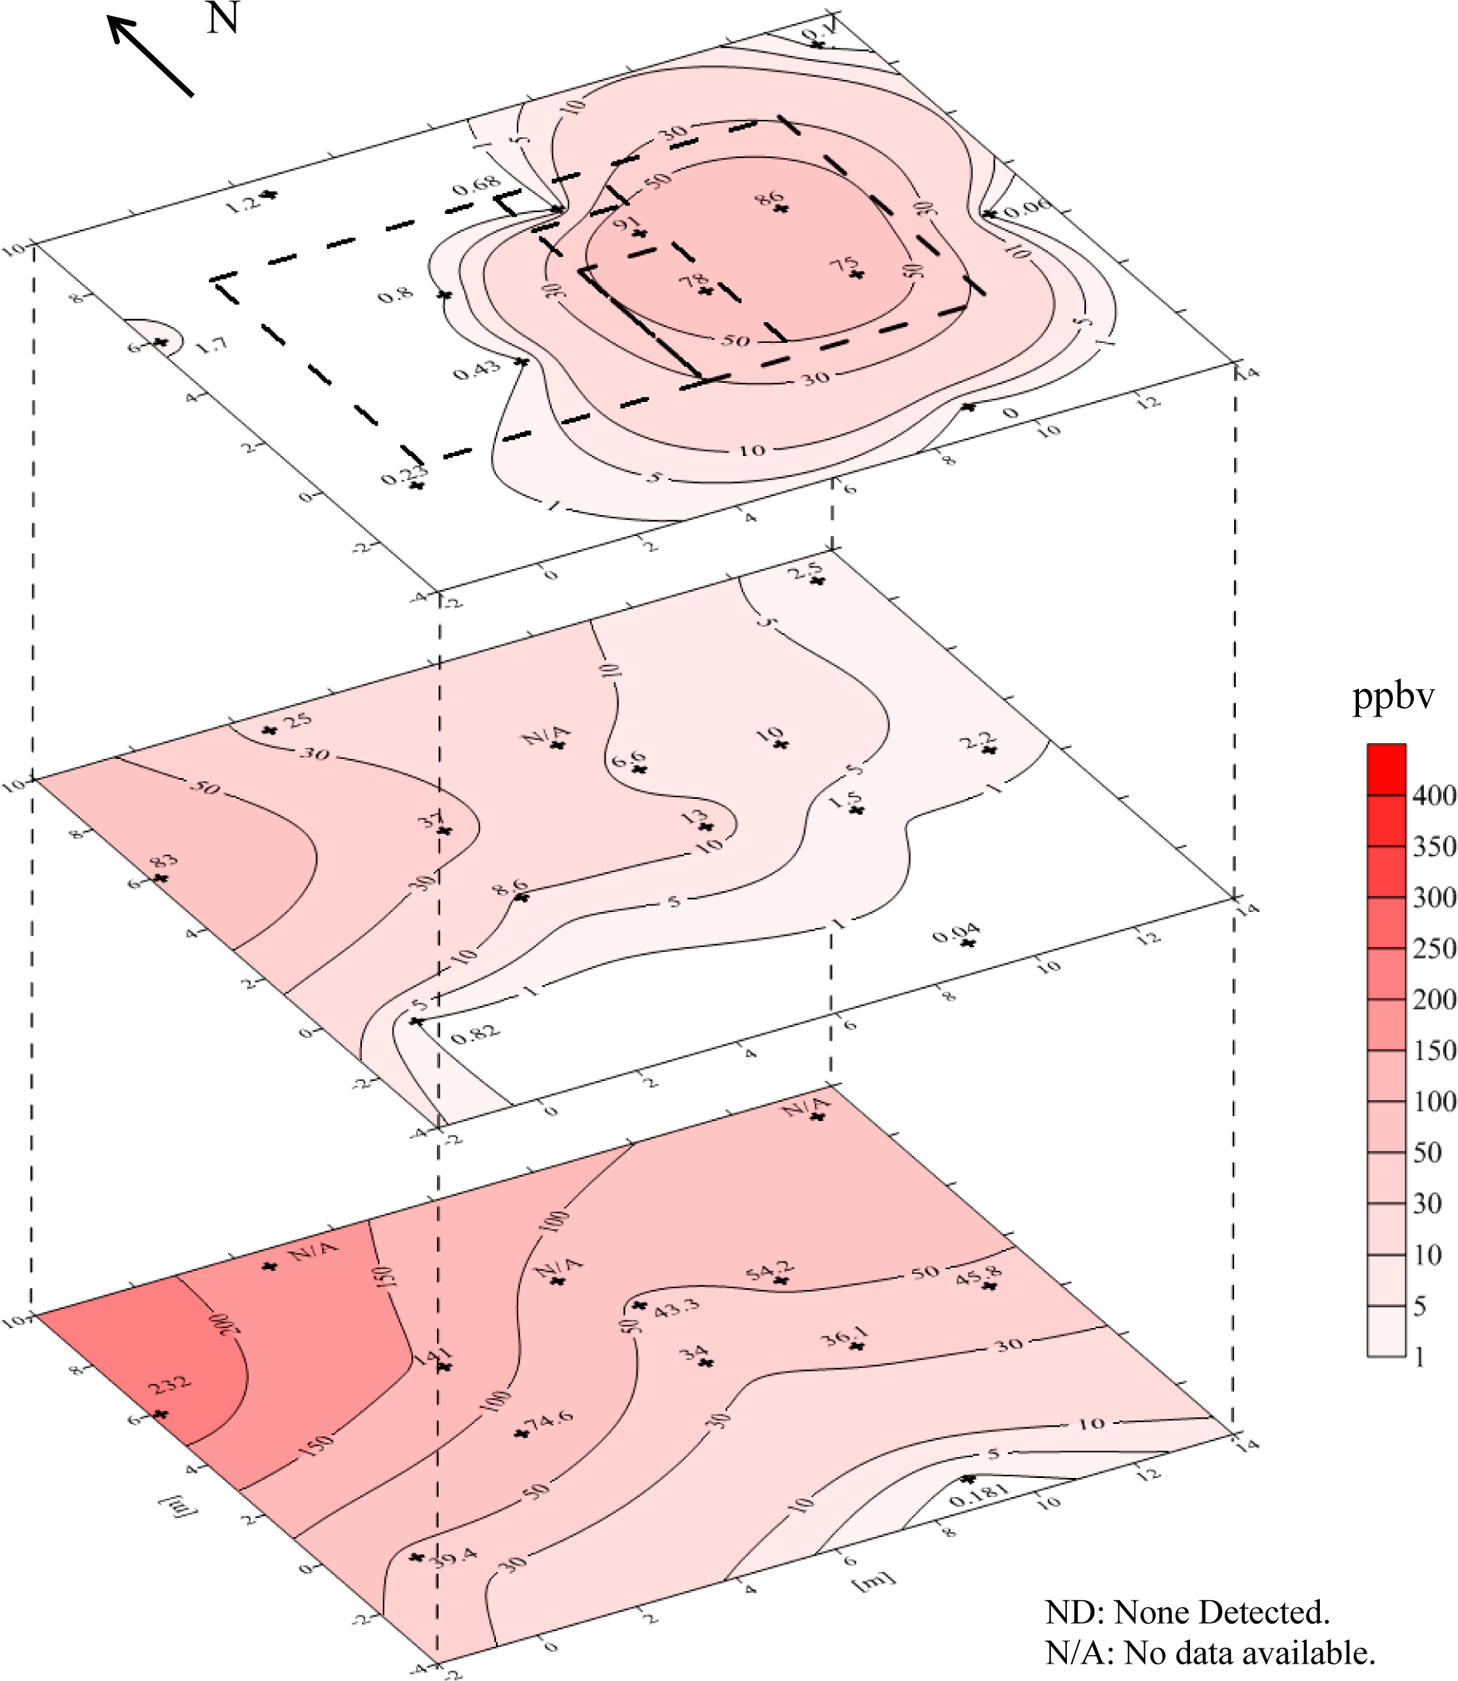
\includegraphics[width=0.85\textwidth]{guo_land_drain_spatial}
  \caption{Distribution of TCE contaminant vapors in the subsurface underneath the ASU house. The top layer is right beneath the foundation, with the two subsequent at \SI{0.9}{\metre} and \SI{1.8}{\metre} below the foundation slab. Snapshot from the period when the CPM system was active. Figure from \citeauthor{guo_identification_2015}\cite{guo_identification_2015}.}
  \label{fig:guo_spatial_variability}
\end{figure}

While this undoubtedly demonstrates the influence of such a preferential pathway on spatial variability, it can be quantitively explored to show just how significant it can be.
To do this, we consider the attenuation from the sub-slab region to the indoor environment
\begin{equation}
  \alpha_\mathrm{subslab} = \frac{c_\mathrm{in}}{c_\mathrm{subslab,5}}
\end{equation}
using sub-slab vapor contaminant concentration data from location 5 (see Figure \ref{fig:asu_house_overview}); this was the sample location closest to exit of the land drain preferential pathway.
These data are visualized in a boxplot in Figure \ref{fig:asu_subslab_attenuation} where we considers the effects of CPM and the land drain preferential pathway on $\alpha_\mathrm{subslab}$.\par

\begin{figure}[htb!]
  \centering
  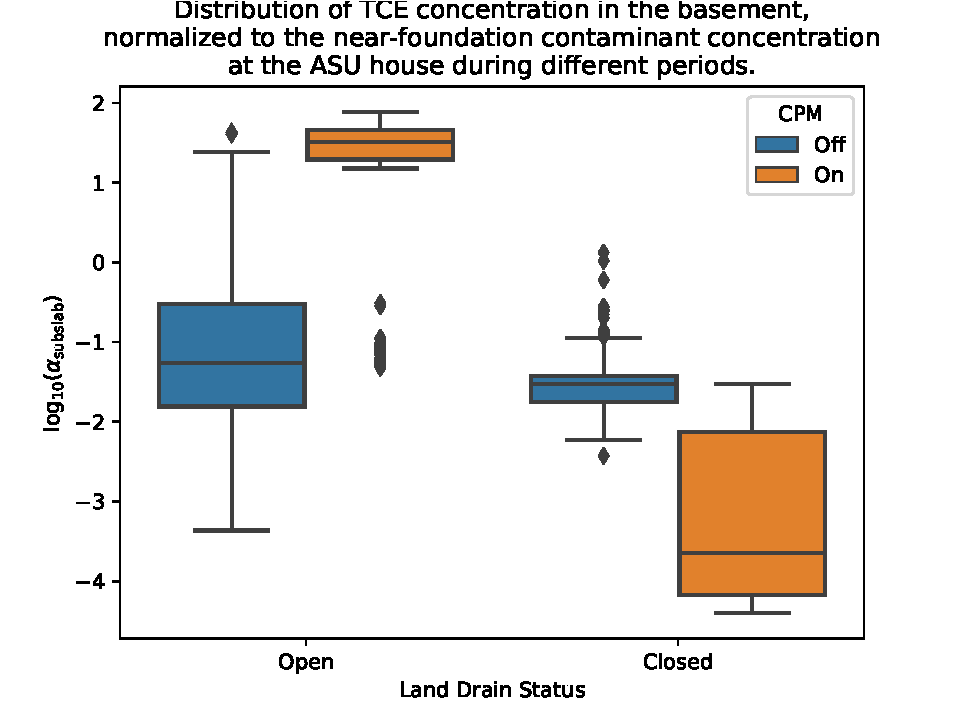
\includegraphics[width=0.85\textwidth]{asu_subslab_attenuation.pdf}
  \caption{Boxplot showing the distribution of $\alpha_\mathrm{subslab}$ considering the effects of CPM and the ASU house land drain preferential pathway. Here $\alpha_\mathrm{subslab}$ is the attenuation from sub-slab sampling location 5 to the indoor environment. The box signifies the interquartile range (IQR) of values, with the central line representing the median value, and the top and bottom of the box are the 25th and 75th percentiles. The whiskers extend to 1.5 times the IQR. Markers indicate outlier data points that fall outside the whiskers.}
  \label{fig:asu_subslab_attenuation}
\end{figure}

Here we that when the preferential pathway was open and the CPM system active, $\alpha_\mathrm{subslab}$ usually exceeds unity by at least an order of magnitude, a situation that should be impossible due to mass conservation; we can likewise see that this is an observed occurrence when the preferential pathway was open by CPM system inactive.
Normally, one would not even expect $\alpha_\mathrm{subslab}$ to be on the order of unity, and looking at the $\alpha_\mathrm{subslab}$ data from the period after the preferential pathway was closed, as well as $\alpha_\mathrm{subslab}$ data collected by the EPA in their VI database, $\alpha_\mathrm{subslab}$ would be expected to range from \num{1e-3} to \num{1e-1} with \num{3e-2} a commonly recognized value\cite{u.s._environmental_protection_agency_oswer_2015}.
Obviously, this is not a violation of mass conservation, but simply an indicator that even though location 5 is only $~\SI{2}{\metre}$ away from the land drain preferential pathway exit, samples taken here clearly fail to capture the highest sub-slab contaminant concentrations; the highest contaminant vapor concentration in the subslab during the preferential pathway open period could  have been order of magnitude higher than recorded.\par

This highlights the large impact that a preferential pathway can have on subsurface spatial contaminant concentration variability.
However, one conclusion from such high $\alpha_\mathrm{subslab}$ values is that they may indicate that there are some indoor contaminant sources present - which was not the situation at the ASU house.
Therefore, this is another aspect of VI that investigators should be cognizant abo ut; very large $\alpha_\mathrm{subslab}$ values could be an indicate an indoor source \textit{or} the existence of some preferential pathway at the VI site.\par

\subsection{EPA Duplex}

\textit{This is purposely left empty for now.}
